%%%%%%%%%%%%%%%%%%%%%%%%%%%%%%%%%%%%%%%%%%%%%%%%%%%%%%%%%%%%%%%%%%%%%%%%%%%%%%%%
% Universität Düsseldorf                                                       %
% Lehrstuhl für Softwaretechnik und Programmiersprachen                        %
% Vorlage für Bachelor- und Masterarbeiten                                     %
% Erstellt: 2019-09-03                                                         %
%%%%%%%%%%%%%%%%%%%%%%%%%%%%%%%%%%%%%%%%%%%%%%%%%%%%%%%%%%%%%%%%%%%%%%%%%%%%%%%%
\documentclass{hhuthesis}
\usepackage[T1]{fontenc}
\usepackage{lmodern}


%%%%%%%%%%%%%%%%%%%%%%%%%%%%%%%%%%%%%%%%%%%%%%%%%%%%%%%%%%%%%%%%%%%%%%%%%%%%%%%%
%% Einstellungen zur Personalisierung                                         %%
%%                                                                            %%
%% Im Folgenden können Sie Ihre Arbeit personalisieren.                       %%
%%%%%%%%%%%%%%%%%%%%%%%%%%%%%%%%%%%%%%%%%%%%%%%%%%%%%%%%%%%%%%%%%%%%%%%%%%%%%%%%

%% Spracheinstellung
%% Kommentieren Sie die entsprechende Zeile ein bzw. aus.
%% Wir empfehlen jedem sich an einer englischen Arbeit zu versuchen.
% \usepackage[ngerman,english]{babel} % English
\usepackage[english,ngerman]{babel} % Deutsch

%% Ihr Name
\author{Vinh Hung Luu}

%% Der Titel der Arbeit
\title{Testpyramide vs. Honeycomb-Modell: Ein Vergleich von Teststrategien im Kontext einer Webanwendung}
% \subtitle{Usually not needed}

%% Der zu erreichende Abschluss, entweder Bachelor oder Master
\graduationtype{Bachelor}
% \graduationtype{Master}

%% Ihr Studienfach
\subject{Informatik}

%% Beginn- und Abgabedaten der Arbeit
\begindate{26.~November~2024} % Beginn
\duedate{26.~Februar~2025} % Abgabe

%% Erst- und Zweitgutachter
\firstexaminer{~Dr.~Jens~Bendisposto}
\secondexaminer{Dr. Markus Brenneis}

%% Farb- oder Schwarzweißdruck
% Benutzen Sie das Kommando \blackwhiteprint,
% wenn sie in schwarzweiß drucken möchten.
% Im Farbdruck ist jede farbige Seite idR teurer.
% \blackwhiteprint % Kommentarzeichen entfernen für Schwarzweißdruck

%%%%%%%%%%%%%%%%%%%%%%%%%%%%%%%%%%%%%%%%%%%%%%%%%%%%%%%%%%%%%%%%%%%%%%%%%%%%%%%%
%% (Ende) Einstellungen zur Personalisierung                                  %%
%%%%%%%%%%%%%%%%%%%%%%%%%%%%%%%%%%%%%%%%%%%%%%%%%%%%%%%%%%%%%%%%%%%%%%%%%%%%%%%%
%% LaTeX Packages in Nutzung                                                  %%
%%                                                                            %%
%% Im folgenden können Sie für die Niederschrift Ihrer Arbeit benötigte       %%
%% LaTeX-Pakete einbinden.                                                    %%
%% Diese Vorlage kommt bereits mit einigen nützlichen inkludierten Paketen.   %%
%%%%%%%%%%%%%%%%%%%%%%%%%%%%%%%%%%%%%%%%%%%%%%%%%%%%%%%%%%%%%%%%%%%%%%%%%%%%%%%%

%% Macht den \todo-Befehl verfügbar.
%% Hiermit können Sie Abschnitte annotieren,
%% welche weiterer Bearbeitung bedürfen.
\usepackage[textsize=scriptsize]{todonotes}

%% Zeige Zeilennummern in der Arbeit an.
%% Der \linenumbers Befehl muss hierzu aufgerufen werden.
%% Praktisch für Feedback Ihrer potentiellen Korrekturleser!
\usepackage{lineno}
% \linenumbers % <- Kommentar entfernen!


%% Häufig benutzte mathematische Packages.
\usepackage{amsfonts}
\usepackage{amsmath}
\usepackage{amssymb}

\usepackage{siunitx} % \num Befehl zum einfacheren Formatieren von Zahlen.
\usepackage{enumitem} % Leichter konfigurierbare enumerate-Umgebungen.
\usepackage{subcaption} % Unterteilung von Figures in Subfigures.
\usepackage[colorlinks]{hyperref} % Klickbare Links (z.B. Inhaltsverzeichnis).
\usepackage[hypcap=true]{caption} % Setzt Hyperref-Links an den Float-Anfang.
\usepackage{xurl} % \url Kommando für Darstellung von Links
\usepackage{csquotes} % Improved quoting.
\usepackage[expansion=false]{microtype}


%% Tabellen
\usepackage{tabularx} % tabularx Umgebung für mehr Kontrolle über Tabellen.
\usepackage{booktabs} % \toprule, \midrule, \bottomrule
\usepackage{multirow}
\usepackage{multicol}
\usepackage{longtable} % Große Tabellen gehen über mehrere Seiten.

%% Quellcode
\usepackage{listings} % Einbindung von Code.

%% Algorithmen in Pseudocode
\usepackage{algorithm} % Float-Umgebung für angegebene Algorithmen.
\usepackage{algorithmicx} % Angabe von Algorithmen in Pseudocode.
\usepackage{algpseudocode} % Standard Pseudocode-Elemente für Algorithmen.

%% Intelligenteres Referenzieren mittels \cref.
%% \languagename um dynamisch zwischen ngerman oder english zu wechseln.
\usepackage[\languagename,capitalize,noabbrev]{cleveref}

%%%%%%%%%%%%%%%%%%%%%%%%%%%%%%%%%%%%%%%%%%%%%%%%%%%%%%%%%%%%%%%%%%%%%%%%%%%%%%%%
%% (Ende) LaTeX Packages in Nutzung                                           %%
%%%%%%%%%%%%%%%%%%%%%%%%%%%%%%%%%%%%%%%%%%%%%%%%%%%%%%%%%%%%%%%%%%%%%%%%%%%%%%%%

\setlength{\parskip}{0pt}
\setlength{\itemsep}{0pt}
\usepackage{setspace}
\setstretch{1.0}
\usepackage{placeins}
\begin{document}

%% Set up title page, declaration of authorship, abstract, acknowledgements
\frontmatter
\makefrontmatter

%%%%%%%%%%%%%%%%%%%%%%%%%%%%%%%%%%%%%%%%%%%%%%%%%%%%%%%%%%%%%%%%%%%%%%%%%%%%%%%%
%% Danksagungen                                                               %%
%%%%%%%%%%%%%%%%%%%%%%%%%%%%%%%%%%%%%%%%%%%%%%%%%%%%%%%%%%%%%%%%%%%%%%%%%%%%%%%%
\begin{acknowledgements}
Ich möchte mich herzlich bei Prof. Dr. Jens Bendisposto für die engagierte Betreuung meiner Bachelorarbeit bedanken. Besonders schätze ich die wertvollen Anregungen und die Unterstützung während der zweiwöchigen Betreuungsphase, die maßgeblich zur Fertigstellung dieser Arbeit beigetragen haben.
\end{acknowledgements}
%%%%%%%%%%%%%%%%%%%%%%%%%%%%%%%%%%%%%%%%%%%%%%%%%%%%%%%%%%%%%%%%%%%%%%%%%%%%%%%%
%% (Ende) Danksagungen                                                        %%
%%%%%%%%%%%%%%%%%%%%%%%%%%%%%%%%%%%%%%%%%%%%%%%%%%%%%%%%%%%%%%%%%%%%%%%%%%%%%%%%
%%%%%%%%%%%%%%%%%%%%%%%%%%%%%%%%%%%%%%%%%%%%%%%%%%%%%%%%%%%%%%%%%%%%%%%%%%%%%%%%
%% Erklärung zur Nutzung generativer KI                                       %%
%%%%%%%%%%%%%%%%%%%%%%%%%%%%%%%%%%%%%%%%%%%%%%%%%%%%%%%%%%%%%%%%%%%%%%%%%%%%%%%%
\clearpage
\section*{Erklärung zur Nutzung generativer KI}
\thispagestyle{plain} 

Im Rahmen dieser Bachelorarbeit wurden generative KI-Tools unterstützend verwendet:

\begin{itemize}
	\item \textbf{ChatGPT} zur sprachlichen Verbesserung von Textabschnitten.  
	\item \textbf{GitHub Copilot und ChatGPT} als Werkzeug zur Unterstützung bei der Code-Entwicklung.  
	\item \textbf{DeepL Write} zur Optimierung der sprachlichen Ausdrucksweise.  
\end{itemize}

Diese Werkzeuge wurden ausschließlich zur sprachlichen und technischen Unterstützung genutzt. Die wissenschaftliche Analyse, Argumentation sowie die erzielten Ergebnisse basieren auf eigener Arbeit.

\clearpage % Erzwingt eine neue Seite
%%%%%%%%%%%%%%%%%%%%%%%%%%%%%%%%%%%%%%%%%%%%%%%%%%%%%%%%%%%%%%%%%%%%%%%%%%%%%%%%
%% (Ende) Erklärung zur Nutzung generativer KI                                %%
%%%%%%%%%%%%%%%%%%%%%%%%%%%%%%%%%%%%%%%%%%%%%%%%%%%%%%%%%%%%%%%%%%%%%%%%%%%%%%%%

\setcounter{tocdepth}{2}
\tableofcontents

%% Listings of figures, tables, etc. Delete what is not needed.
\clearpage
\listoftables\thispagestyle{headings}
\listoffigures
\listofalgorithms % Algorithms
\lstlistoflistings % Code Listings

\mainmatter

%%%%%%%%%%%%%%%%%%%%%%%%%%%%%%%%%%%%%%%%%%%%%%%%%%%%%%%%%%%%%%%%%%%%%%%%%%%%%%%%
%% Der Inhalt der Arbeit                                                      %%
%%                                                                            %%
%% Hier können Sie die schriftliche Ausarbeitung ihrer Arbeit                 %%
%% niederschreiben. Der Übersicht halber bietet sich jedoch an, dies in einer %%
%% oder mehreren separaten Dateien zu tun, welche mittels \input eingebunden  %%
%% werden --- wie auch in der Vorlage geschieht.                              %%
%%%%%%%%%%%%%%%%%%%%%%%%%%%%%%%%%%%%%%%%%%%%%%%%%%%%%%%%%%%%%%%%%%%%%%%%%%%%%%%%

%%%%%%%%%%%%%%%%%%%%%%%%%%%%%%%%%%%%%%%%%%%%%%%%%%%%%%%%%%%%%%%%%%%%%%%%%%%%%%%%
% Diese Datei beinhaltet den eigentlichen Inhalt Ihrer Arbeit.
%
% Es bietet sich der Übersicht halber an, die einzelnen Abschnitte jeweils
% in eigene Dateien zu schreiben und mittels \input einzubinden.
% Eine mögliche Verzeichnisstruktur sähe entsprechend so aus:
%
%     thesis/
%     +- tex/
%     |  +- introduction.tex
%     |  +- motivation.tex
%     |  +- experiments.tex
%     |  |  ...
%     |  +- conclusion.tex
%     +- abstract.tex
%     +- contents.tex
%     +- thesis.tex
%%%%%%%%%%%%%%%%%%%%%%%%%%%%%%%%%%%%%%%%%%%%%%%%%%%%%%%%%%%%%%%%%%%%%%%%%%%%%%%%

\section{Einleitung}

\subsection{Motivation}
Im Modul \emph{ProgrammierPraktikum 2} wurde Test-Driven Development (TDD) eingeführt. Dabei erhielt ich erstmals Einblicke in praktische Teststrategien, insbesondere in die \emph{Testpyramide}. Als Anfänger faszinierten mich die klare Struktur und die methodische Vorgehensweise. Dies veranlasste mich dazu, die Frage zu stellen, ob dieser Ansatz universell angewendet wird oder ob alternative Modelle existieren.

Aus meinem aktuellen Werkstudentenjob ergab sich eine weitere Beobachtung. In einigen Projekten werden vorwiegend Systemtests implementiert, die das Gesamtverhalten der Anwendung abdecken. Separate Unit-Tests für einzelne Schichten kommen dabei weitgehend zu kurz. Diese Beobachtung bezieht sich ausschließlich auf mein derzeitiges Arbeitsumfeld und lässt keine Rückschlüsse auf allgemeine Entwicklungen in der Softwareentwicklung zu.
Darüber hinaus wurde in fachlichen Diskussionen eine von Spotify genutzte Teststrategie~\cite{Spotify18} erörtert, die als Honeycomb-Modell bekannt ist. Diese unterschiedlichen Erfahrungen und Beobachtungen bilden den Ausgangspunkt dieser Arbeit. Es soll untersucht werden, welche Vor- und Nachteile die Testpyramide und das Honeycomb-Modell im Kontext einer Webanwendung bieten.


\subsection{Ziel der Arbeit}
Diese Arbeit vergleicht die Effektivität der Testpyramide und des Testing-Honeycomb-Modells. Dazu wird eine Webanwendung entwickelt, in der mit Test-Driven Development implementiert wurde. Die Anwendung dient als Plattform für die Organisation und Kommunikation zwischen Veranstaltern und Schaustellern. Sie umfasst Module wie das Bewerbungsmanagement, das Vertragsmanagement und das Veranstaltungsmanagement. Veranstalter können Veranstaltungen erstellen, während Schausteller sich bewerben und Verträge abschließen.  Zudem wurde Spring Security integriert, um ein Sicherheitskonzept zu realisieren. Es wird evaluiert, welcher Ansatz hinsichtlich Testqualität, Laufzeit und Komplexit\"at Vorteile bietet. Zur Messung der Testabdeckung werden JaCoCo und PIT eingesetzt. Weiterhin wird untersucht, wie sich der Einsatz einer H2-Datenbank im Vergleich zu produktionsnahen Datenbanken mit Testcontainers auswirkt. Die Ergebnisse dienen als Grundlage f\"ur praxisnahe Empfehlungen.

\subsection{Aufbau der Arbeit}
Die Arbeit ist in mehrere Kapitel gegliedert. Zunächst werden die theoretischen Grundlagen zu Teststrategien, Datenbanktechnologien und Evaluierungstools dargelegt. Im Anschluss wird die Methodik vorgestellt, welche den generellen Ablauf der Untersuchung beschreibt. 

Im Hauptteil der Arbeit wird schrittweise anhand einzelner Features der Webanwendung vorgegangen. Für jedes Feature werden zunächst beide Teststrategien implementiert und deren Laufzeiten gemessen. Die gewonnenen Erfahrungen und Beobachtungen werden dabei dokumentiert und analysiert. Anschließend werden sicherheitsrelevante Aspekte untersucht, bevor die Frontend-Seiten implementiert werden. Danach erfolgt die Einführung von Spring Security, wobei zusätzliche Tests ergänzt werden, falls bestimmte Funktionen zuvor nicht berücksichtigt wurden und nochmal gemessen.

Den Abschluss bildet eine Zusammenfassung der experimentellen Ergebnisse sowie ein Ausblick auf zukünftige Entwicklungen im Bereich der Softwaretests.

\section{Grundlagen der Testmethodik}
Ein strukturierter Ansatz für Softwaretests ist entscheidend, um Anwendungen systematisch auf Fehler zu überprüfen und deren Stabilität zu gewährleisten.

In diesem Abschnitt werden die Testpyramide und das Testing-Honeycomb-Modell vorgestellt. Beide Modelle sind in der Praxis etabliert und bieten unterschiedliche Perspektiven auf die Organisation von Tests.

\subsection{Testpyramide}
Die Testpyramide wurde erstmals von Fowler~\cite{Fow12} als hierarchisches Modell eingeführt. Sie gliedert Softwaretests typischerweise in drei Hauptkategorien: Unit-Tests, Integrationstests und Systemtests. In manchen Darstellungen wird die Pyramide durch eine vierte Ebene ergänzt, die manuelle Tests umfasst. Das Modell verfolgt das Ziel, die Mehrheit der Tests auf den unteren Ebenen anzusiedeln, da diese schneller ausführbar und kosteneffizienter sind.

\begin{itemize}
	\item \textbf{Unit-Tests:} Die Basis der Pyramide bilden Unit-Tests. Sie testen einzelne, isolierte Softwareeinheiten wie Methoden oder Klassen. Durch die Unabhängigkeit von externen Schnittstellen ermöglichen sie eine schnelle und einfache Fehlerlokalisierung bei geringer Komplexität~\cite{BF14}.
	\item \textbf{Integrationstests:} Diese Ebene konzentriert sich auf das Zusammenspiel mehrerer Module oder Komponenten. Obwohl sie mehr Aufwand in der Implementierung erfordern, stellen sie sicher, dass die Integration der einzelnen Teile reibungslos funktioniert~\cite{Wac15}.
	\item \textbf{Systemtests:} An der Spitze der Pyramide stehen Systemtests. Sie überprüfen das gesamte System auf funktionale und nicht-funktionale Anforderungen. Aufgrund ihrer hohen Komplexität und Kosten sollten sie gezielt und sparsam eingesetzt werden~\cite{BF14}.
\end{itemize}

Cohn~\cite{Coh09} hebt hervor, dass Tests möglichst auf der niedrigsten Ebene implementiert werden sollten, um Kosten und Laufzeiten gering zu halten. Wacker~\cite{Wac15} ergänzt, dass Systemtests zwar notwendig sind, aber in ihrer Anzahl begrenzt bleiben sollten, um die Effizienz der Testpipeline nicht zu beeinträchtigen.

\subsection{Honeycomb}

Das Honeycomb-Modell wurde von Spotify~\cite{Spotify18} speziell für Microservices-Architekturen entwickelt. Es legt den Schwerpunkt auf Integrationstests, da die größte Komplexität in solchen Architekturen häufig in der Interaktion zwischen den Diensten liegt. Spotify betont, dass diese Tests nicht nur die Kommunikation zwischen Services, sondern auch die zugrunde liegende Infrastruktur, wie Datenbanken und APIs, umfassen sollten, um realitätsnahe Szenarien abzubilden~\cite{Spotify18}.

In ihrem Artikel \enquote{Testing of Microservices} beschreibt Spotify diesen Ansatz mit den Worten: \begin{quote} \enquote{We spin up a database, populate it, start the service, and query the actual API in the tests.} \end{quote} Dieses Zitat zeigt, dass Spotify eine vollständige Testumgebung aufsetzt, allerdings in einer kontrollierten Umgebung (z. B. mit einer lokalen Testdatenbank oder Testcontainers). Dies unterscheidet sich von klassischen integrierten Tests, da die externe Abhängigkeit hier simuliert wird, anstatt eine produktive API oder ein echtes externes System zu nutzen.

Spotify~\cite{Spotify18} beschreibt im Rahmen des Honeycomb-Modells drei zentrale Testtypen:  
\begin{itemize} 
	\item \textbf{Integrationstests:} Diese bilden den Kern des Modells und stellen sicher, dass die Schnittstellen innerhalb eines Systems korrekt implementiert sind und die Zusammenarbeit zwischen internen Komponenten erwartungsgemäß funktioniert~\cite{Spotify18}. Beispielsweise kann ein Integrationstest überprüfen, ob ein REST-Controller die erwarteten Antworten liefert, wenn er mit dem Service-Layer kommuniziert. 
	\item \textbf{Implementierungsdetail-Tests:} Diese Tests konzentrieren sich auf die interne Logik eines einzelnen Services, beispielsweise komplexe Berechnungen. Spotify betrachtet sie als Ergänzung zu Integrationstests, ordnet ihnen jedoch eine geringere Priorität zu~\cite{Spotify18}. 
	\item \textbf{Integrierte Tests:} Diese Tests überprüfen die Funktionalität eines Systems unter Berücksichtigung externer Abhängigkeiten, beispielsweise durch die Anbindung an andere Microservices, Datenbanken oder APIs. Da sie von der Verfügbarkeit und der korrekten Funktion dieser externen Systeme abhängen, sind sie fehleranfällig. Laut Spotify sollten sie möglichst reduziert oder vermieden werden, da sie die Wartung erschweren, die Testpipeline verlangsamen und zu Fehlinterpretationen von Testergebnissen führen können~\cite{Spotify18}. Ein Beispiel für einen integrierten Test wäre die Validierung der Kommunikation eines Microservices mit einer externen Zahlungs-API, bei der API-Ausfälle zu unerwarteten Testergebnissen führen können.
\end{itemize}

Dieses Zitat zeigt, dass Spotify eine vollständige Testumgebung aufsetzt, allerdings in einer kontrollierten Umgebung z. B. mit einer lokalen Testdatenbank oder Testcontainers. Dies unterscheidet sich von klassischen integrierten Tests, da die externe Abhängigkeit hier simuliert wird, anstatt eine produktive API oder ein echtes externes System zu nutzen.

Gleichzeitig warnt Spotify jedoch ausdrücklich vor der Nutzung sogenannter integrierter Tests:  
\begin{quote}
	\enquote{That means we should focus on Integration Tests, have a few Implementation Detail Tests and even fewer Integrated Tests (ideally none).}~\cite{Spotify18}
\end{quote}
Das Honeycomb-Modell priorisiert Integrationstests, um die Interaktionspunkte innerhalb eines Systems umfassend zu prüfen. Spotify empfiehlt dabei, Tests in einer vollständig kontrollierten Umgebung durchzuführen, anstatt auf produktive externe Abhängigkeiten zurückzugreifen~\cite{Spotify18}.

Obwohl Spotify integrierte Tests mit unkontrollierten externen Abhängigkeiten kritisch sieht, setzen sie dennoch auf realitätsnahe Testumgebungen, die unter vollständiger Kontrolle des Testsystems bleiben. Beispielsweise kann hierfür eine eigene Testdatenbank aufgesetzt werden, ohne dass ein direkter Zugriff auf produktive Systeme erforderlich ist.

Auch in dieser Arbeit wird weitgehend auf Mocking verzichtet, insbesondere für die Datenbank, indem eine produktionsnahe Testumgebung mit Testcontainers verwendet wird. Dies ermöglicht eine realitätsnahe Überprüfung des Zusammenspiels aller Komponenten, ohne dabei auf unzuverlässige externe Abhängigkeiten angewiesen zu sein.


\subsection{Datenbanklösung für Tests}

In dieser Arbeit werden die H2-Datenbank und eine MySQL-Datenbank mithilfe von Testcontainers implementiert. Die Wahl der Datenbank richtet sich nach der jeweiligen Teststrategie.

Im Rahmen der Testpyramide kommen beide Datenbanklösungen zum Einsatz. Klassische Unit-Tests werden vollständig isoliert von einer Datenbank ausgeführt, indem Mocking-Techniken eingesetzt werden. Die H2-Datenbank~\cite{H2Doc} wird hingegen für Integrationstests verwendet, da sie eine einfache Konfiguration und kurze Laufzeiten ermöglicht. Sie erlaubt die Prüfung der Datenzugriffsschicht ohne Abhängigkeit von einer externen Datenbankinstanz. Ergänzend wird für umfassendere Integrationstests eine MySQL-Datenbank mithilfe von Testcontainers eingesetzt. Diese ermöglicht realitätsnahe Tests in einer produktionsnahen Umgebung und minimiert das Risiko von Umgebungsinkonsistenzen~\cite{Testcontainers}.


Das Honeycomb-Modell setzt ausschließlich auf die MySQL-Datenbank mit Testcontainers. Ziel ist es, realistische Testbedingungen zu schaffen, indem das gesamte System einschließlich der Datenbank getestet wird~\cite{Spotify18}. Testcontainers stellt eine produktionsnahe Umgebung bereit und bildet Interaktionen zwischen Anwendung und Datenbank realistisch ab. Zur Sicherstellung eines konsistenten Datenbankschemas wird Flyway als Migrationstool eingesetzt~\cite{FlywayDoc}.

Die gewählte Kombination erlaubt es, die Vorteile beider Ansätze zu nutzen. Die H2-Datenbank ermöglicht schnelle, ressourcenschonende Tests in der Testpyramide, während Testcontainers realitätsnahe Tests unterstützt und für das Honeycomb-Modell unverzichtbar ist.
Die Wahl der Teststrategie basiert auf den Anforderungen der Webanwendung Venow, die als Fallstudie dient. Durch den Einsatz von H2 und Testcontainers werden die zuvor beschriebenen Testansätze praktisch erprobt, um die Systemfunktionen wie den Bewerbungsprozess, die Vertragsverwaltung und der Veranstaltungsverwaltung umfassend zu validieren.

\section{Webanwendung zur Veranstaltungsorganisation}

Die entwickelte Webanwendung unterstützt Veranstalter und Schausteller bei der Organisation von Events. Veranstalter können eigenständig Events erstellen, Bewerbungen verwalten und Verträge abschließen. Schausteller haben die Möglichkeit, sich über die Plattform für Events zu bewerben und ihre Teilnahme zu organisieren.

\subsection{Motivation für die Wahl der Webanwendung als Fallstudie}

Diese Webanwendung wurde als Fallstudie gewählt, weil sie mehrere zentrale Herausforderungen der Softwareentwicklung abbildet. Die Plattform erfasst komplexe organisatorische Abläufe. Sie unterstützt Veranstalter bei der Verwaltung von Events und Schausteller bei der Bewerbung und Vertragsabwicklung. Beide Nutzergruppen haben unterschiedliche, aber miteinander verknüpfte Interaktionen mit dem System. Die Anwendung bietet vielfältige Testfälle, um verschiedene Teststrategien systematisch zu vergleichen. Durch ihre praxisnahe Umsetzung dient sie als reales Beispiel für die digitale Transformation im Veranstaltungsmanagement.

Ein persönlicher Grund für die Entwicklung dieser Webanwendung war eine reale Erfahrung. Ein Bekannter berichtete, dass er jedes Jahr seinen Foodtruck für eine Veranstaltung anmelden musste. Der Bewerbungsprozess verlief ausschließlich analog. Er musste den Veranstalter kontaktieren, viele E-Mails schreiben und zahlreiche Telefonate führen. Die vertraglichen Details wurden ebenfalls manuell geklärt. Dieser Prozess war aufwendig und fehleranfällig. Es war schwierig, den Überblick über alle Bewerbungen und abgeschlossenen Verträge zu behalten. Daraus entstand die Idee, eine digitale Lösung zu entwickeln. Eine Plattform sollte alle Bewerbungen und Verträge zentral speichern. Der Bewerbungsprozess sollte mit wenigen Klicks erfolgen. Verträge sollten direkt digital erstellt und verwaltet werden. Veranstalter sollten neue Events effizient organisieren können. Viele Veranstaltungen sind weiterhin analog und verfügen über keine zentrale digitale Lösung. Diese Webanwendung bietet eine einheitliche Plattform für Veranstalter und Schausteller.

\subsection{Bewerbungsprozess}

Schausteller können sich über vorhandene Events informieren und sich direkt über die Plattform bewerben. Veranstalter können die eingegangenen Bewerbungen einsehen und den aktuellen Status jeder Bewerbung nachverfolgen. Das System zeigt an, ob eine Bewerbung neu eingereicht, akzeptiert oder bereits in einen Vertrag überführt wurde. Wird eine Bewerbung angenommen, kann der Veranstalter daraus einen Vertrag generieren.

\begin{figure}[h]
	\centering
	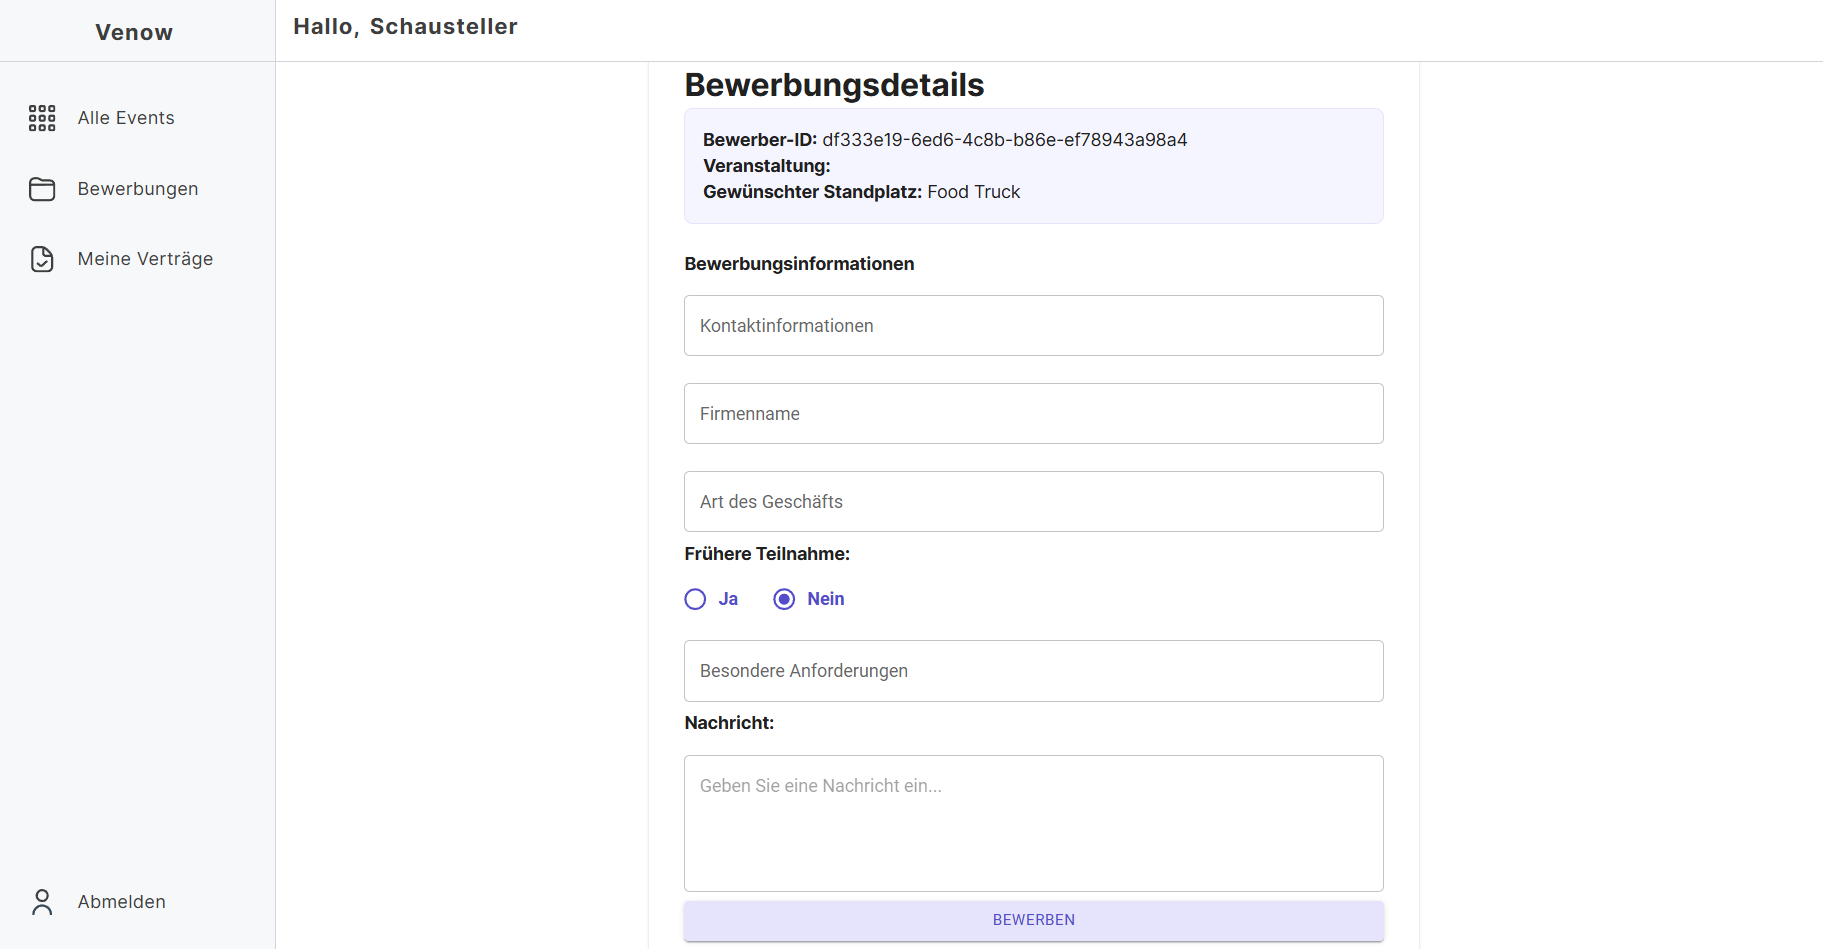
\includegraphics[width=0.8\textwidth]{fig/frontend-exhibitor-apply.png}
	\caption{Bewerbungsformular für Schausteller}
	\label{fig:exhibitor-apply}
\end{figure}

\subsection{Vertragsverwaltung}

Veranstalter können aus einer angenommenen Bewerbung einen Vertrag erstellen. Dabei werden Details wie Preis und Standplatznummer festgelegt. Schausteller erhalten den Vertrag digital und können diesen einsehen. Sie haben die Möglichkeit, den Vertrag zu akzeptieren oder abzulehnen. Sobald beide Parteien den Vertrag annehmen, ist der Bewerbungsprozess abgeschlossen.

\begin{figure}[h]
	\centering
	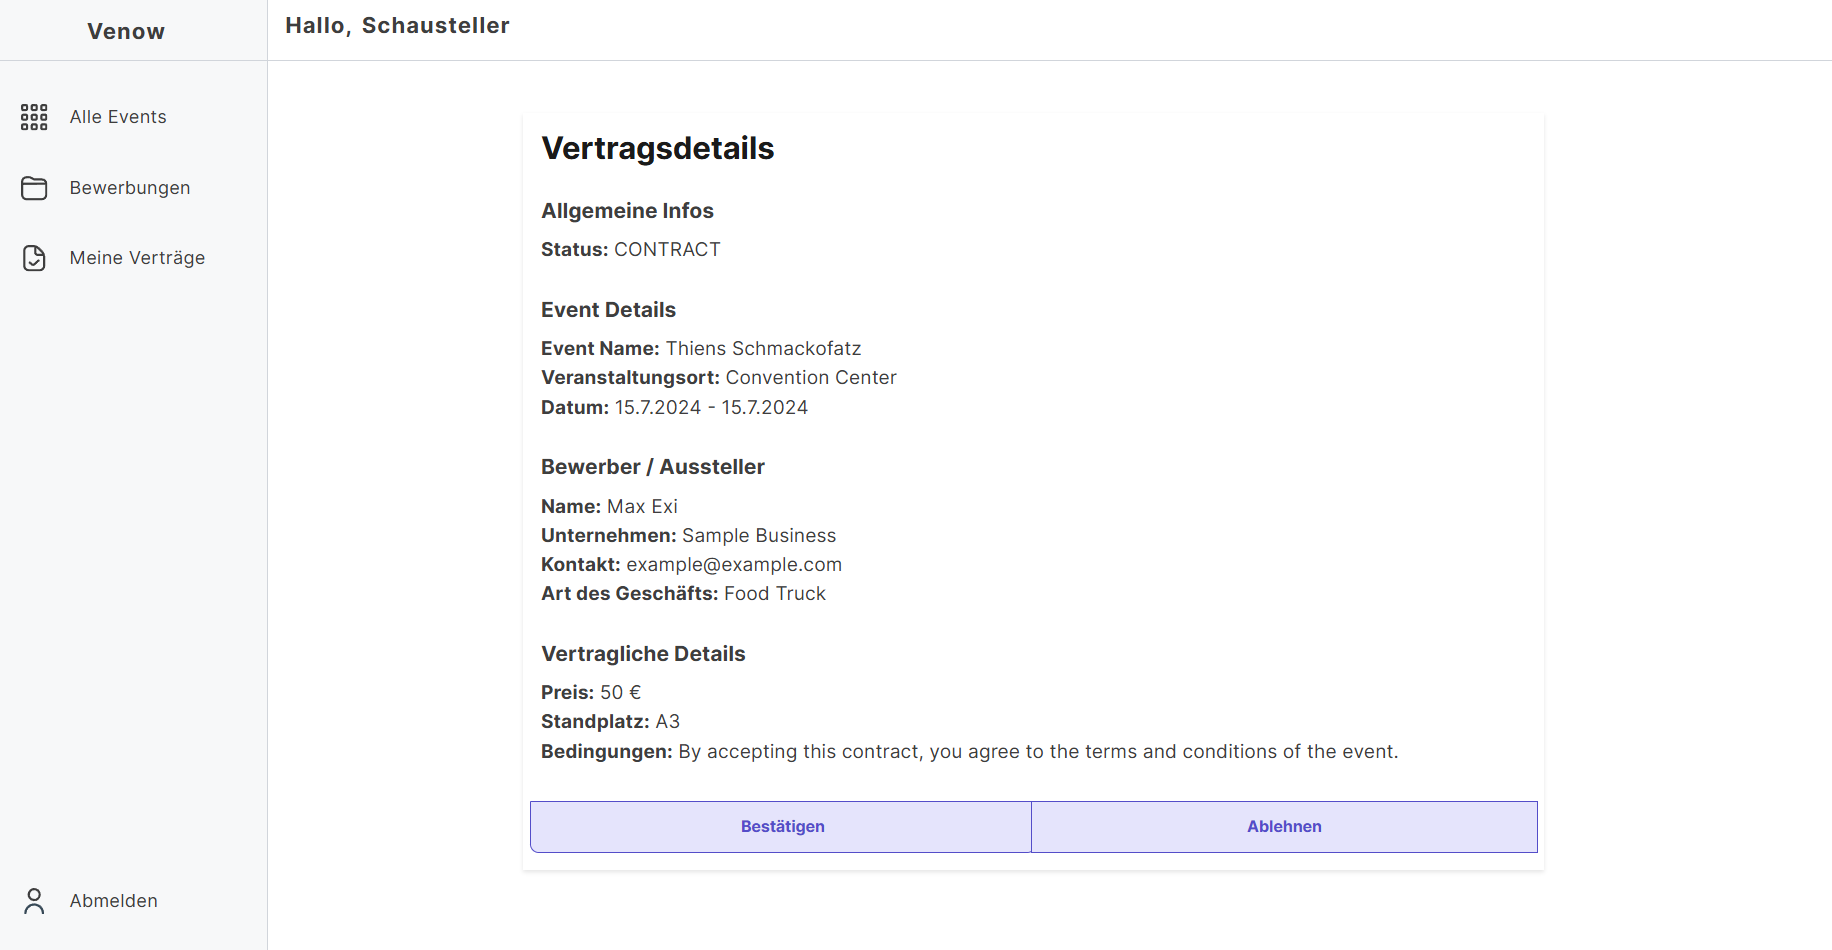
\includegraphics[width=0.8\textwidth]{fig/frontend-exhibitor-contracts-confirm.png}
	\caption{Vertragsdetails für Schausteller}
	\label{fig:exhibitor-contracts}
\end{figure}

\subsection{Veranstaltungs-Management}

Veranstalter können neue Veranstaltungen erstellen und bestehende Veranstaltungen bearbeiten. Alle Veranstaltungen sind für Schausteller sichtbar. Eine integrierte Suchfunktion ermöglicht es, gezielt nach Events zu suchen. Veranstalter können relevante Veranstaltungsdaten wie Datum, Ort und verfügbare Standplätze erfassen. Diese Informationen sind mit anderen Modulen verknüpft. Alle Prozessschritte greifen ineinander, um eine effiziente Verwaltung zu ermöglichen.

\begin{figure}[h]
	\centering
	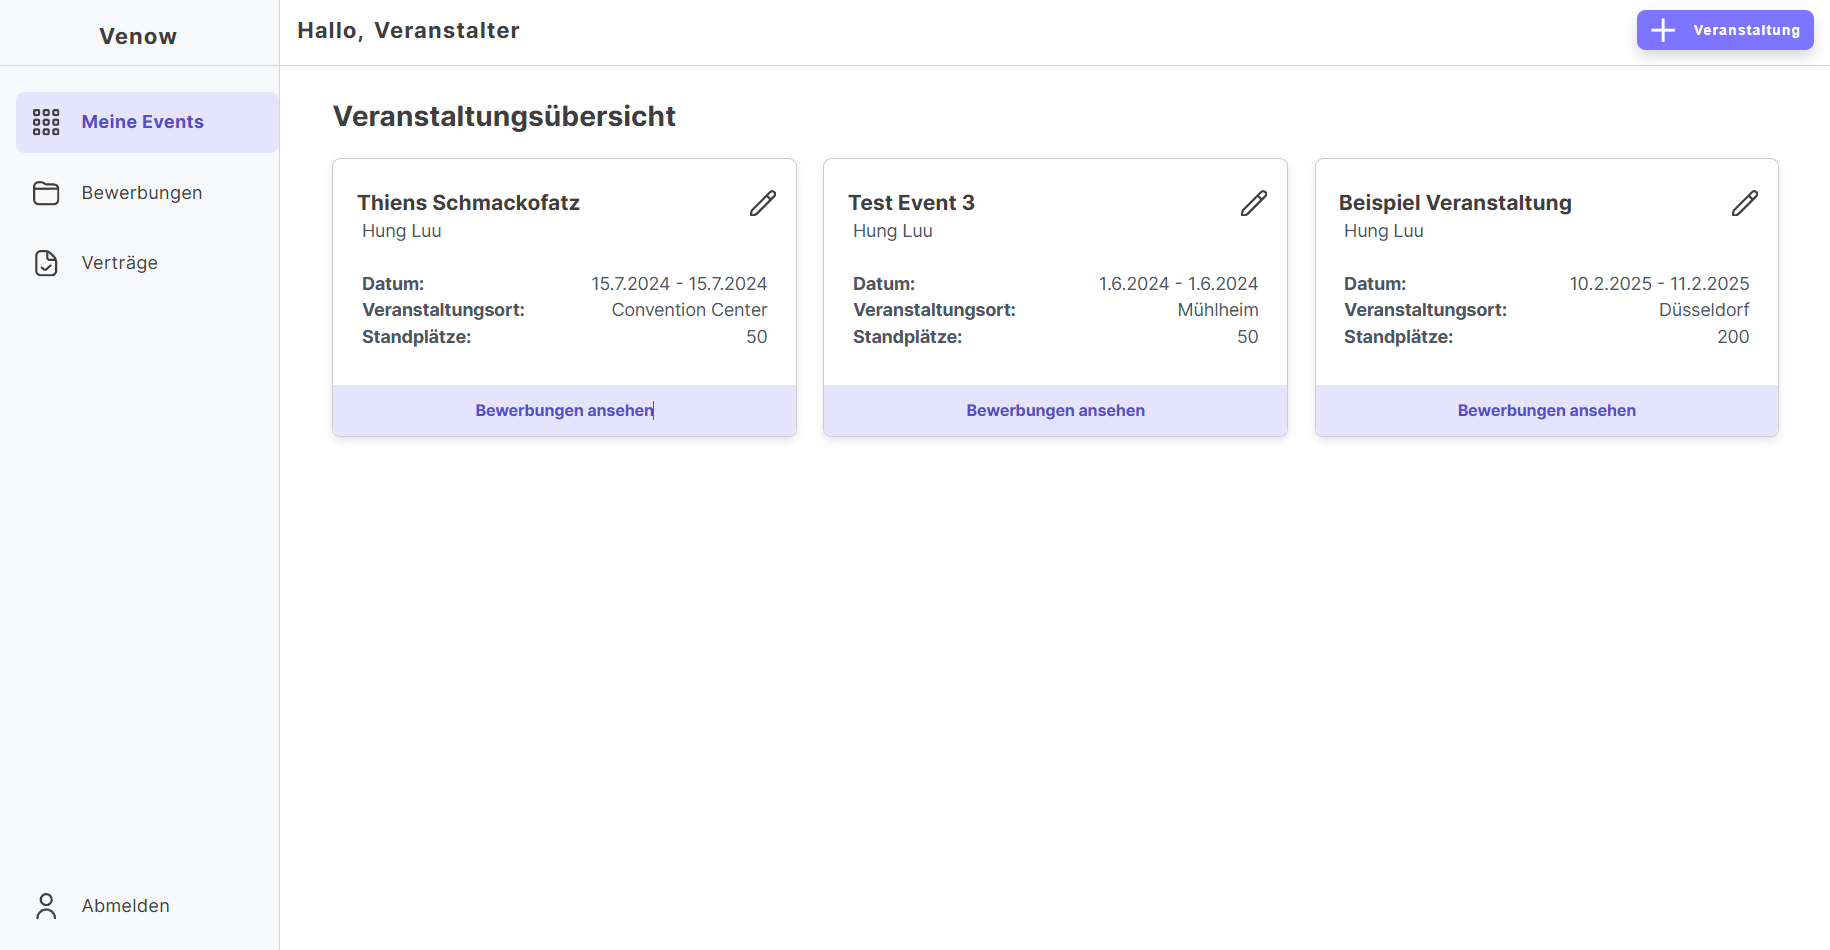
\includegraphics[width=0.8\textwidth]{fig/frontend-organizer-events.png}
	\caption{Übersicht der Events für Veranstalter}
	\label{fig:organizer-events}
\end{figure}

\subsection{Bewerbungen verwalten und Verträge erstellen}

Veranstalter können Bewerbungen prüfen und über eine Annahme oder Ablehnung entscheiden. Wird eine Bewerbung angenommen, kann der Veranstalter direkt einen Vertrag über die Plattform erstellen.

\begin{figure}[h]
	\centering
	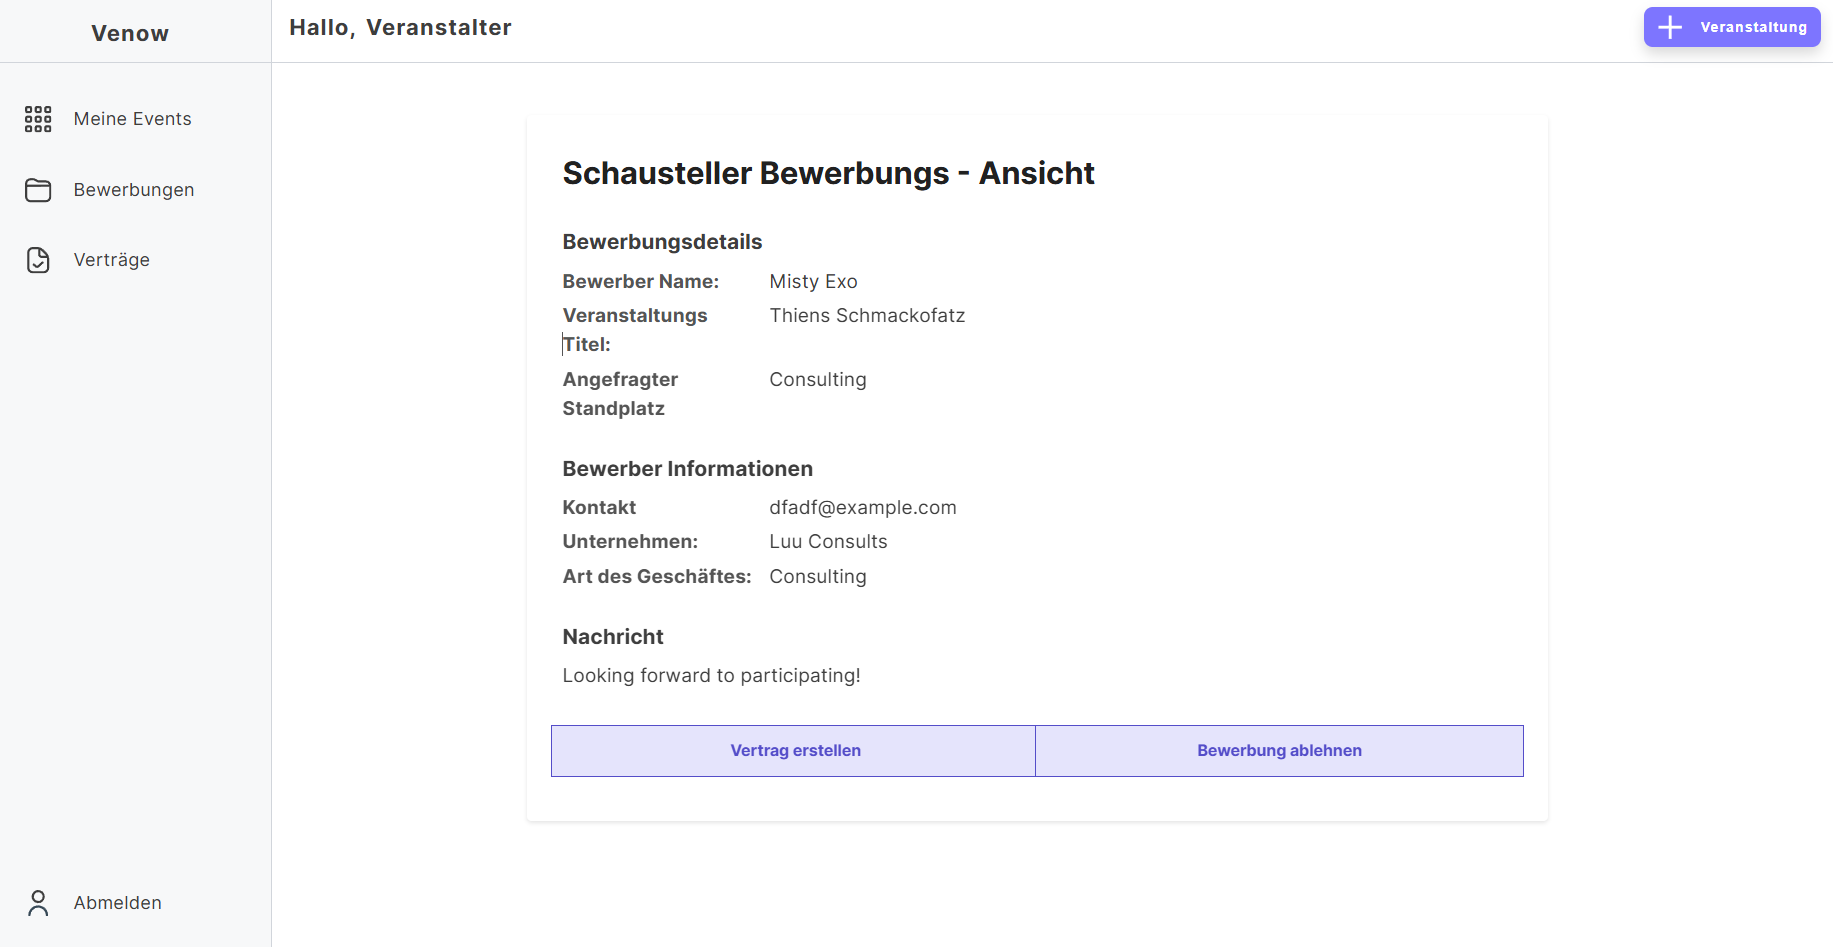
\includegraphics[width=0.8\textwidth]{fig/frontend-organizer-applications-create-contract.png}
	\caption{Ansicht einer Bewerbung mit der Möglichkeit zur Vertragserstellung}
	\label{fig:applications-create-contract}
\end{figure}

\subsection{Erstellung von Events durch Veranstalter}

Veranstalter haben die Möglichkeit, über ein strukturiertes Formular neue Events anzulegen. Hier können sie alle relevanten Informationen wie Datum, Standort und verfügbare Stellplätze erfassen.

\begin{figure}[h]
	\centering
	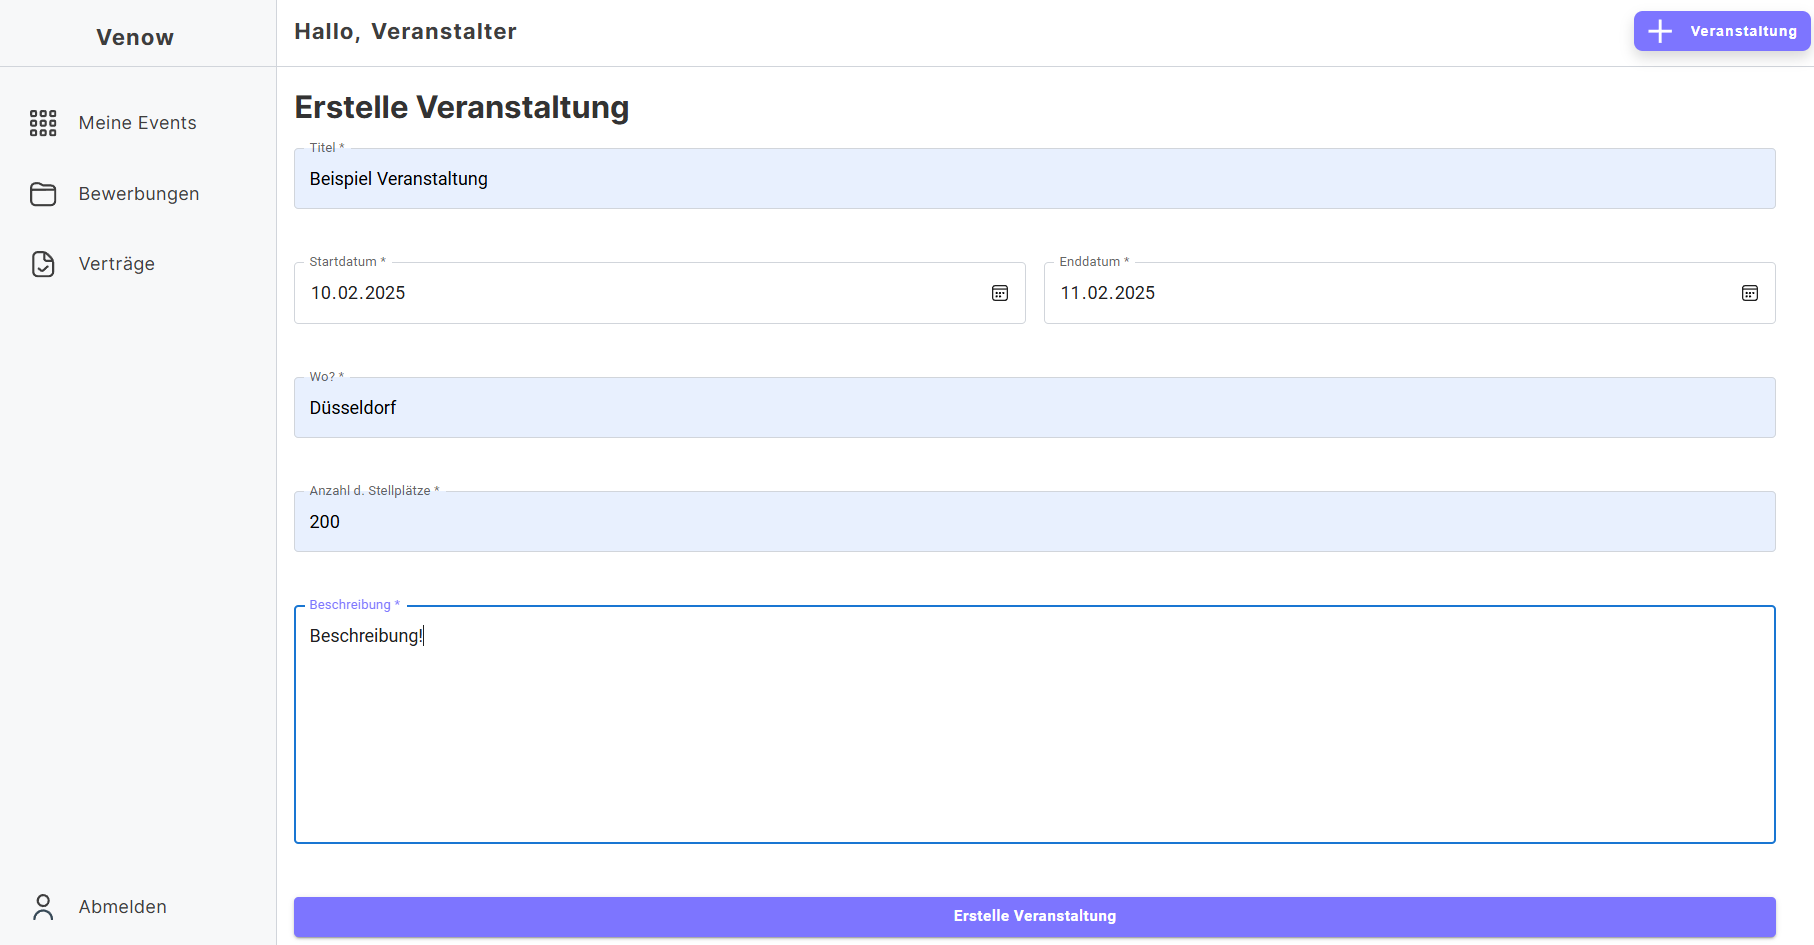
\includegraphics[width=0.8\textwidth]{fig/frontend-organizer-events-create.png}
	\caption{Formular zur Event-Erstellung durch Veranstalter}
	\label{fig:organizer-events-create}
\end{figure}

\subsection{Login-Funktion und grundlegendes Veranstaltungsmanagement}

Die Webanwendung enthält eine Login-Funktion, die den Zugriff auf registrierte Nutzer beschränkt. Dadurch wird sichergestellt, dass nur autorisierte Personen Bewerbungen und Verträge verwalten können. Veranstalter können ihre Veranstaltungen kontinuierlich aktualisieren. Die Plattform stellt sicher, dass alle Prozesse digital und nachvollziehbar bleiben.
Die detaillierte Beschreibung dieser Anwendungsfälle bildet die Grundlage für die spätere Analyse der Teststrategien. Insbesondere wird untersucht, wie sich die Implementierung der verschiedenen Module auf die Effizienz und Effektivität der Tests auswirkt.

\section{Methodik}

\subsection{Entwicklung von Testszenarien}

\subsection{Tests für spezifische Anwendungsfälle}

\subsection{Datenanalyse und empirische Auswertung}
\section{Durchführung und Ergebnisse}

\subsection{Vergleich der Teststrategien anhand spezifischer Anwendungsfälle}
Die beiden Teststrategien \texttt{Testpyramide} und \texttt{Honeycomb-Modell} wurden anhand praxisnaher Anwendungsfälle evaluiert. Die Analyse umfasst den Bewerbungsprozess, das Vertragsmanagement und das Eventmanagement. Die Messungen (Laufzeit, Anzahl durchgeführter Tests) sowie die Testabdeckung (vgl. Abschnitte \ref{tab:jacoco-ergebnisse} und \ref{tab:pitest-detailed-logs}) wurden in einer einheitlichen Testumgebung durchgeführt, um die Ergebnisse vergleichbar zu halten. 

\subsubsection{Bewerbungsprozess}
Im Bewerbungsprozess zeigte sich, dass die \texttt{Testpyramide} durch die Verwendung einer H2-Datenbank geringere Laufzeiten aufweist, während das \texttt{Honeycomb-Modell} mehr Zeit in Integrationspfade investiert und dabei MySQL-Testcontainer nutzt. Die Ergebnisse sind in Tabelle \ref{tab:bewerbungsprozess} dargestellt.

\begin{table}[h]
	\centering
	\caption{Laufzeiten und Testanzahl im Bewerbungsprozess}
	\label{tab:bewerbungsprozess}
	\begin{tabular}{|l|l|l|l|l|}
		\hline
		\textbf{Modell} & \textbf{Test Typ} & \textbf{Laufzeit} & \textbf{Anzahl der Tests} & \textbf{Datenbank} \\
		\hline
		Honeycomb       & Integration       & \textbf{1 s 582 ms} & 18  & Testcontainer MySQL \\
		\hline
		Testpyramide    & Alle              & \textbf{1 s 876 ms} & 44  & H2 \\
		\hline
		Testpyramide    & Alle              & \textbf{3 s 408 ms} & 44  & Testcontainer MySQL \\
		\hline
	\end{tabular}
\end{table}

\subsubsection{Vertragsmanagement}
Das Vertragsmanagement, als zentraler und vergleichsweise aufwendiger Anwendungsfall, zeigt deutliche Unterschiede zwischen den Strategien. Tabelle \ref{tab:vertragsmanagement} veranschaulicht, dass das \texttt{Honeycomb-Modell} infolge umfangreicher Integrationstests mit MySQL länger läuft, während die \texttt{Testpyramide} kürzere Zeiten bei einer größeren Testanzahl verzeichnet.

\begin{table}[h]
	\centering
	\caption{Laufzeiten und Testanzahl im Vertragsmanagement}
	\label{tab:vertragsmanagement}
	\begin{tabular}{|l|l|l|l|l|}
		\hline
		\textbf{Modell} & \textbf{Test Typ} & \textbf{Laufzeit} & \textbf{Anzahl der Tests} & \textbf{Datenbank} \\
		\hline
		Honeycomb       & Integration       & \textbf{9 s 835 ms} & 48  & Testcontainer MySQL \\
		\hline
		Testpyramide    & Alle              & \textbf{2 s 565 ms} & 103 & H2 \\
		\hline
		Testpyramide    & Alle              & \textbf{3 s 757 ms} & 103 & Testcontainer MySQL \\
		\hline
	\end{tabular}
\end{table}

\subsubsection{Eventmanagement}
Beim Eventmanagement werden komplexe Datenbankvorgänge und mehrere miteinander interagierende Module getestet. Tabelle \ref{tab:eventmanagement} belegt, dass das \texttt{Honeycomb-Modell} im Integrationsmodus nochmals mehr Laufzeit benötigt als die \texttt{Testpyramide}, die wiederum mit einer H2-Datenbank besonders schnelle Durchläufe erzielt.

\begin{table}[h]
	\centering
	\caption{Laufzeiten und Testanzahl im Eventmanagement}
	\label{tab:eventmanagement}
	\begin{tabular}{|l|l|l|l|l|}
		\hline
		\textbf{Modell} & \textbf{Test Typ} & \textbf{Laufzeit} & \textbf{Anzahl der Tests} & \textbf{Datenbank} \\
		\hline
		Honeycomb       & Integration       & \textbf{12 s 939 ms} & 58  & Testcontainer MySQL \\
		\hline
		Testpyramide    & Alle              & \textbf{2 s 858 ms}  & 140 & H2 \\
		\hline
		Testpyramide    & Alle              & \textbf{7 s 428 ms}  & 140 & Testcontainer MySQL \\
		\hline
	\end{tabular}
\end{table}

\subsection{Zusammenfassung der Testabdeckung mit JaCoCo}
Um die Teststrategien \texttt{Testpyramide} und \texttt{Honeycomb-Modell} hinsichtlich ihrer Abdeckung zu bewerten, wurde das Tool \texttt{JaCoCo} eingesetzt. Es erfasst verschiedene Metriken (z.\,B. \texttt{Instructions}, \texttt{Branches}, \texttt{Methods} und \texttt{Classes}) und ermöglicht eine Differenzierung, wie viele Teile des Codes (in Zeilen und Verzweigungen) von den Tests durchlaufen werden. Die Resultate sind in Tabelle \ref{tab:jacoco-ergebnisse} zu sehen.

\begin{table}[h]
	\centering
	\caption{Testabdeckung mit JaCoCo für Honeycomb-Modell und Testpyramide}
	\label{tab:jacoco-ergebnisse}
	\begin{tabular}{|l|l|l|}
		\hline
		\textbf{Metrik}       & \textbf{Honeycomb} & \textbf{Testpyramide} \\ \hline
		Instructions          & 91 \%              & 94 \%                 \\ \hline
		Branches              & 65 \%              & 80 \%                 \\ \hline
		Lines                 & 91 \% (Missed: 51) & 94 \% (Missed: 35)    \\ \hline
		Methods               & 87.6 \%            & 91.1 \%               \\ \hline
		Classes               & 98 \%              & 100 \%                \\ \hline
	\end{tabular}
\end{table}

Die Messungen zeigen, dass beide Ansätze eine insgesamt hohe Codeabdeckung erzielen. Während die \texttt{Testpyramide} in den meisten Metriken leicht vorn liegt (z.\,B. \texttt{Branches}, \texttt{Methods}), stellt das \texttt{Honeycomb-Modell} mit weniger Tests eine ebenfalls hohe Abdeckung sicher, vor allem in \texttt{Instructions} (91\,\%) und \texttt{Classes} (98\,\%).

\subsection{Mutation Testing mit PITest}
Zur Beurteilung, wie gut die Tests nicht nur \emph{Code ausführen}, sondern auch \emph{Fehler aufdecken} können, kam \texttt{PITest} zum Einsatz. Dieses Werkzeug generiert Mutationen (z.\,B. veränderte Return-Werte oder Negation von Bedingungen), um zu prüfen, ob sie von den Tests entdeckt und „getötet“ werden.

\subsubsection{Ergebnisse der Mutation Tests}
Tabelle \ref{tab:pitest-detailed-logs} zeigt exemplarisch, wie viele Mutationen (\texttt{Gen.}) pro Mutator erzeugt, getötet (\texttt{Killed}) und u.\,U. ohne Abdeckung (\texttt{NoCov}) geblieben sind. Überlebende Mutationen (\texttt{Surv.}) geben Aufschluss über mögliche Lücken in den existierenden Tests. 

\begin{table}[h!]
	\centering
	\caption{Detaillierte PITest-Log-Daten im Vergleich (Honeycomb vs.\ Testpyramide)}
	\label{tab:pitest-detailed-logs}
	\resizebox{\textwidth}{!}{%
		\begin{tabular}{|l||c|c|c|c|c||c|c|c|c|c|}
			\hline
			\multirow{2}{*}{\textbf{Mutator}} 
			& \multicolumn{5}{c||}{\textbf{Honeycomb-Modell}} 
			& \multicolumn{5}{c|}{\textbf{Testpyramide}} \\
			\cline{2-11}
			& \textbf{Gen.} & \textbf{Killed(\%)} & \textbf{Surv.} & \textbf{TOut} & \textbf{NoCov} 
			& \textbf{Gen.} & \textbf{Killed(\%)} & \textbf{Surv.} & \textbf{TOut} & \textbf{NoCov} \\
			\hline
			\textbf{ConditionalsBoundary} & 2 & 2 (100\,\%) & 0 & 2 & 0 
			& 2 & 1 (50\,\%)  & 1 & 0 & 0 \\
			\textbf{PrimitiveReturns}     & 1 & 1 (100\,\%) & 0 & 1 & 0
			& 1 & 1 (100\,\%) & 0 & 0 & 0 \\
			\textbf{VoidMethodCall}       & 9 & 8 (89\,\%)  & 0 & 6 & 1
			& 9 & 8 (89\,\%)  & 1 & 0 & 0 \\
			\textbf{BooleanTrueReturnVals}& 4 & 4 (100\,\%) & 0 & 4 & 0
			& 4 & 4 (100\,\%) & 0 & 0 & 0 \\
			\textbf{NullReturnVals}       & 78 & 68 (87\,\%) & 0 & 61 & 10
			& 78 & 72 (92\,\%) & 0 & 3 & 6 \\
			\textbf{EmptyObjectReturnVals}& 19 & 19 (100\,\%) & 0 & 19 & 0
			& 19 & 18 (95\,\%)  & 0 & 2 & 1 \\
			\textbf{BooleanFalseReturnVals} & 5 & 5 (100\,\%) & 0 & 5 & 0
			& 5 & 4 (80\,\%)  & 1 & 0 & 0 \\
			\textbf{NegateConditionals}     & 33 & 31 (94\,\%) & 0 & 31 & 2
			& 33 & 33 (100\,\%)& 0 & 1 & 0 \\
			\hline
		\end{tabular}
	}
\end{table}

\paragraph{Zusammenfassung der wichtigsten Kennzahlen}
\begin{itemize}
	\item \textbf{Honeycomb-Modell:}
	\begin{itemize}
		\item Generierte Mutationen: 151
		\item Getötete Mutationen: 138 (91\,\%)
		\item Mutationen ohne Abdeckung (NO\_COVERAGE): 13
		\item Line Coverage (mutierte Klassen): 92\,\% (495/537)
		\item Test Strength: 100\,\% (alle abgedeckten Mutationen wurden getötet)
		\item Timeouts: 129
		\item Gesamtlaufzeit: ca. 52 Minuten 21 Sekunden
	\end{itemize}
	\item \textbf{Testpyramide:}
	\begin{itemize}
		\item Generierte Mutationen: 151
		\item Getötete Mutationen: 141 (93\,\%)
		\item Mutationen ohne Abdeckung (NO\_COVERAGE): 7
		\item Line Coverage (mutierte Klassen): 94\,\% (507/537)
		\item Test Strength: 98\,\% (141/144 abgedeckte Mutationen wurden getötet)
		\item Timeouts: 6
		\item Gesamtlaufzeit: ca. 5 Minuten 25 Sekunden
	\end{itemize}
\end{itemize}

\begin{table}[h]
	\centering
	\caption{Kompakte Gegenüberstellung der Hauptmetriken (Honeycomb vs.\ Testpyramide)}
	\label{tab:pittest-ergebnisse}
	\begin{tabular}{|l|c|c|}
		\hline
		\textbf{Metrik} & \textbf{Honeycomb} & \textbf{Testpyramide} \\
		\hline
		Line Coverage (mutierte Klassen) & 92\,\% (495/537) & 94\,\% (507/537) \\
		\hline
		Mutation Coverage & 91\,\% (138/151) & 93\,\% (141/151) \\
		\hline
		Mutationen ohne Abdeckung (NO\_COVERAGE) & 13 & 7 \\
		\hline
		Überlebende Mutationen (SURVIVED) & 0 & 3 \\
		\hline
		Test Strength & 100\,\% (138/138) & 98\,\% (141/144) \\
		\hline
		Timeouts & 129 & 6 \\
		\hline
		Tests pro Mutation & 0{,}01 & 1{,}08 \\
		\hline
		Gesamtlaufzeit & 52 Min 21 Sek & 5 Min 25 Sek \\
		\hline
	\end{tabular}
\end{table}

\subsubsection{Zusammenfassung der Mutation-Testergebnisse}
Die in Tabelle \ref{tab:pittest-ergebnisse} aufgeführten Metriken machen deutlich, dass beide Strategien eine hohe Mutation Coverage aufweisen. Das \texttt{Honeycomb-Modell} benötigt jedoch mehr Zeit (rund 52 Minuten) und verzeichnet 129 Timeouts. Die \texttt{Testpyramide} führt zwar mehr Einzeltests aus, schliesst ihre Durchläufe jedoch in knapp 5\,Minuten ab und weist deutlich weniger Timeouts auf. 

\subsection{Vergleich der Datenbanklösungen}
Der Einsatz einer H2-Datenbank führt zu \emph{kürzeren} Testlaufzeiten und ist in vielen Fällen für Unit- und (kleinere) Integrationstests ausreichend schnell. Testcontainer-basierte MySQL-Instanzen bilden hingegen \emph{produktionsnähere Bedingungen} ab, was jedoch in komplexeren Szenarien höhere Laufzeiten und potenziell mehr Timeouts nach sich zieht. Beide Ansätze können je nach Zielsetzung miteinander kombiniert werden, um ein ausgewogenes Verhältnis aus Geschwindigkeit und Realitätsnähe zu erreichen.

\subsection{Zusammenfassung der Ergebnisse}
Die durchgeführten Tests in den drei Anwendungsfällen – Bewerbungsprozess, Vertragsmanagement und Eventmanagement – zeigen, dass das \texttt{Honeycomb-Modell} und die \texttt{Testpyramide} jeweils charakteristische Laufzeiten, Testumfänge und Abdeckungswerte aufweisen. Anhand der JaCoCo-Metriken (Tabelle \ref{tab:jacoco-ergebnisse}) ist erkennbar, dass beide Strategien hohe Codeabdeckung liefern, wobei die \texttt{Testpyramide} in den meisten Kennzahlen (z.\,B. Branch-Coverage) noch etwas weiter reicht. Die Messungen mit \texttt{PITest} (Tabellen \ref{tab:pitest-detailed-logs} und \ref{tab:pittest-ergebnisse}) bestätigen, dass beide Ansätze Mutationen effektiv erkennen und töten können, wenngleich sich \emph{Laufzeit} und \emph{Anzahl der Timeouts} deutlich unterscheiden. 

H2 ermöglicht bei vielen Tests eine sehr kurze Durchlaufzeit, während MySQL-Testcontainer realistischere Datenbankszenarien und damit umfassendere Integrationsprüfungen erlauben. In allen drei Fällen (Bewerbungsprozess, Vertragsmanagement, Eventmanagement) waren die Laufzeiten beim \texttt{Honeycomb-Modell} länger, häufig bei vergleichsweise wenigen Tests. Die \texttt{Testpyramide} zeigte mehr Einzeltests und kürzere Gesamtdauer, insbesondere mit H2. Somit bleibt festzuhalten, dass beide Strategien je nach Einsatzzweck – \emph{Realitätsnähe} versus \emph{Schnelligkeit und Detailtiefe} – sinnvoll eingesetzt werden können.

\section{Schlussfolgerungen und Empfehlungen}
Die durchgeführte Analyse der Teststrategien Testpyramide und Testing Honeycomb Modell hat gezeigt, dass beide Ansätze spezifische Vor- und Nachteile mit sich bringen. Während die Testpyramide durch ihre modulare Struktur eine höhere Testgeschwindigkeit und gezieltere Fehlerdiagnose ermöglicht, bietet das Testing Honeycomb Modell eine realistischere Abbildung der Systeminteraktionen, geht jedoch mit höheren Laufzeiten und einem komplexeren Debugging Prozess einher. 

Die Messungen zeigen, dass die Testpyramide insgesamt eine drei Mal schnellere Testdurchführung bietet, während das Testing Honeycomb Modell eine um fünfzehn Prozent höhere Systemabdeckung erreicht. Besonders auffällig ist die erhöhte Anzahl an Tests in der Testpyramide, da diese Strategie kleinere Codeeinheiten isoliert testet, während das Testing Honeycomb Modell vollständige End to End Abläufe prüft.  

Die Testpyramide erleichtert durch ihre schichtweise getesteten Komponenten die gezielte Fehlerdiagnose. Probleme können frühzeitig auf Methoden oder Serviceebene erkannt werden. Das Testing Honeycomb Modell erfordert oft eine vollständige Analyse des Anwendungsflusses, um Fehler zu lokalisieren. Dies macht Debugging deutlich aufwendiger. Besonders in der Mapper Schicht zeigte sich, dass Fehler in der Testpyramide schnell identifiziert wurden, während sie im Testing Honeycomb Modell nur durch tiefgehende Log Analysen auffindbar waren.  

Die Einführung von Spring Security hat in beiden Modellen zu einer erhöhten Anzahl an Testfällen und längeren Laufzeiten geführt. Während die Testpyramide durch ihren modularen Aufbau besser mit den zusätzlichen Sicherheitsprüfungen umgehen konnte, führten sie im Testing Honeycomb Modell zu einer deutlichen Laufzeitsteigerung. Die Ergebnisse zeigen, dass zusätzliche Sicherheitsmechanismen in End to End Tests erheblichen Overhead erzeugen und ihre Auswirkungen frühzeitig berücksichtigt werden sollten.  

Die Wahl der Datenbank hat ebenfalls eine signifikante Rolle gespielt. Tests mit H zwei liefen deutlich schneller als mit MySQL Testcontainern. Allerdings gab es Kompatibilitätsprobleme bei SQL Syntax und Fremdschlüsselvalidierungen. Besonders auffällig war die unterschiedliche Interpretation von Escape Zeichen und Fremdschlüssel Checks zwischen H zwei und MySQL, die zu unerwartetem Verhalten in Tests führten. MySQL Testcontainer bieten eine realitätsnähere Umgebung, benötigen jedoch signifikant längere Initialisierungszeiten, was insbesondere im Testing Honeycomb Modell problematisch war.  

Beim Testing Honeycomb Modell konnte durch Test Driven Development zunächst mit einem einzigen Test begonnen werden, ohne direkt Service oder Repository Klassen zu implementieren. Die Testpyramide erfordert eine schrittweise Implementierung der Schichten, erlaubt aber eine stabilere Codebasis und eine schnellere Testausführung. Nachzüglertests, also Tests die nachträglich hinzugefügt wurden, zeigten, dass die Testpyramide eine bessere Integration neuer Tests ermöglichte, während Testing Honeycomb Tests häufiger vollständig überarbeitet werden mussten.  

Die Ergebnisse legen nahe, dass eine hybride Teststrategie die Stärken beider Modelle kombinieren könnte. Eine mögliche Lösung wäre die Nutzung von Unit Tests und gezielten Integrationstests aus der Testpyramide für schnelle Entwicklungszyklen. Zusätzlich könnten End to End Tests aus dem Testing Honeycomb Modell für komplexe geschäftsprozessorientierte Abläufe integriert werden. Eine adaptive Teststrategie wäre ebenfalls eine Möglichkeit, um je nach Codeänderung automatisch die passende Testmethode auszuwählen.  

Zukünftige Arbeiten könnten sich darauf konzentrieren, wie eine automatisierte Auswahl der Teststrategie entwickelt werden kann, um je nach Systemänderung effizientere Testmechanismen einzusetzen. Eine weitere Optimierung der Datenbankkonfiguration könnte helfen, die Performance von MySQL Testcontainern zu verbessern und Escape Syntax Probleme zu minimieren. Ebenso könnte die detaillierte Untersuchung hybrider Testmodelle zeigen, wie Unit und Integrationstests mit End to End Tests kombiniert werden können, um eine bessere Balance zwischen Effizienz und Systemabdeckung zu erreichen.  

Die Wahl der Teststrategie sollte immer kontextabhängig erfolgen. Die Testpyramide eignet sich besonders für modularen Code und agile Entwicklungsprozesse, bei denen schnelle Rückmeldungen benötigt werden. Das Testing Honeycomb Modell bietet Vorteile für komplexe Systeminteraktionen, erfordert jedoch einen höheren Laufzeitaufwand. Eine Kombination beider Ansätze könnte langfristig eine effiziente und skalierbare Teststrategie ermöglichen, die sowohl die Testabdeckung als auch die Testgeschwindigkeit optimiert.  

Diese Arbeit liefert eine praxisnahe Evaluierung beider Testmodelle und zeigt auf, wie hybride Teststrategien zur Effizienzsteigerung und Fehlerprävention beitragen können.  


\subsection{Zusammenfassung der Ergebnisse je Anwendungsfall}
\subsection{Empfehlungen für den praktischen Einsatz der Teststrategien und Datenbanklösungen}
\subsection{Limitationen und zukünftige Arbeiten}  

Die durchgeführte Untersuchung beschränkt sich auf eine monolithische Architektur mit einer begrenzten Anzahl an Features. Zukünftige Arbeiten könnten untersuchen, wie sich die Teststrategien auf komplexere Geschäftsprozesse auswirken, insbesondere wenn zusätzliche Funktionalitäten integriert werden.  

Ein Aspekt, der in dieser Arbeit nicht behandelt wurde, ist die Anwendung des Testing Honeycomb Modells in einer Microservices Architektur. Eine Studie von Spotify \cite{
Spotify18} beschreibt, dass in Microservices Umgebungen End to End Tests eine zentrale Rolle spielen, da sie sicherstellen, dass die Kommunikation zwischen den unabhängigen Diensten zuverlässig funktioniert.  

Microservices sind ein Architekturstil, bei dem eine Anwendung in mehrere unabhängige Dienste unterteilt wird, die über Netzwerkschnittstellen interagieren. Diese Definition basiert auf den Arbeiten von Fowler und Lewis \cite{fowler2014} sowie Newman \cite{newman2015}, die Microservices als lose gekoppelte, eigenständig deploybare Einheiten beschreiben. Besonders in verteilten Systemen, in denen Services synchron über REST APIs oder asynchron über Messaging Systeme kommunizieren, ergeben sich besondere Herausforderungen bei der Testbarkeit. Während Unit und Integrationstests die isolierte Geschäftslogik eines einzelnen Services validieren, erfassen sie nicht potenzielle Fehler in der Kommunikation zwischen den Services. Das Testing Honeycomb Modell könnte in solchen Szenarien vorteilhaft sein, da es die gesamte Service Interaktion unter realistischen Bedingungen überprüft.  

Die Testergebnisse legen nahe, dass die Testpyramide für kleine bis mittelgroße monolithische Anwendungen eine effiziente Teststrategie darstellt. Sie ermöglicht eine gezielte Fehlerdiagnose und eine hohe Testabdeckung einzelner Komponenten. Mit zunehmender Größe eines Monolithen steigt jedoch die Anzahl der internen Abhängigkeiten, was die Testwartung erschwert. Zudem kann das Testing Honeycomb Modell bei sehr großen Monolithen zu unverhältnismäßig langen Testlaufzeiten führen. Dies deutet darauf hin, dass ab einer bestimmten Komplexitätsstufe eine Aufteilung in Microservices sinnvoll sein könnte, um die Testbarkeit zu verbessern.  

Ein vielversprechender Forschungsansatz könnte die Kombination der Testpyramide mit dem Testing Honeycomb Modell sein. Eine mögliche Strategie wäre die Nutzung der Testpyramide für isolierte Unit- und Integrationstests, um Fehler frühzeitig zu erkennen, während das Testing Honeycomb Modell gezielt für kritische Geschäftsprozesse eingesetzt wird. Anstatt das gesamte System in jedem Testdurchlauf vollständig zu validieren, könnten selektive Honeycomb-Tests durchgeführt werden, um Laufzeiten zu optimieren.  

Zukünftige Arbeiten könnten sich darauf konzentrieren, adaptive Teststrategien zu entwickeln, die je nach Art der Codeänderung automatisch zwischen granularen Tests der Testpyramide und umfassenden Systemtests des Testing Honeycomb Modells entscheiden. Besonders relevant wäre eine genauere Untersuchung, wie Testcontainer optimiert werden können, um Laufzeiten zu reduzieren und gleichzeitig eine hohe Testabdeckung sicherzustellen. Darüber hinaus könnte erforscht werden, inwiefern eine hybride Teststrategie für Microservices anwendbar ist, bei der die Testpyramide innerhalb einzelner Services genutzt wird und das Testing Honeycomb Modell für Service-übergreifende Tests zum Einsatz kommt.  

\section{Fazit und Ausblick}
\subsection{Zusammenfassung der Arbeit}
\subsection{Mögliche Erweiterung}
\subsection{Zukünftige Forschung}
%% Dieser Part kann auskommentiert werden, sollte kein Anhang nötig sein.
%% Der \appendix-Befehl leitet hierbei den Anhang ein.
 \appendix
 \section{Hilfsmittel}
In dieser Arbeit wurden die folgenden Hilfsmittel genutzt:

\begin{itemize}
	\item Code-Editor: Intellij / TeXstudio
	\item Programmiersprachen: Java, TypeScript
	\item Datenbank: MySQL mit Testcontainers, H2
	\item Frameworks: Spring Boot, React
\end{itemize}

\clearpage

\section{Zusätzliche Abbildungen}

\begin{figure}[h]
	\centering
	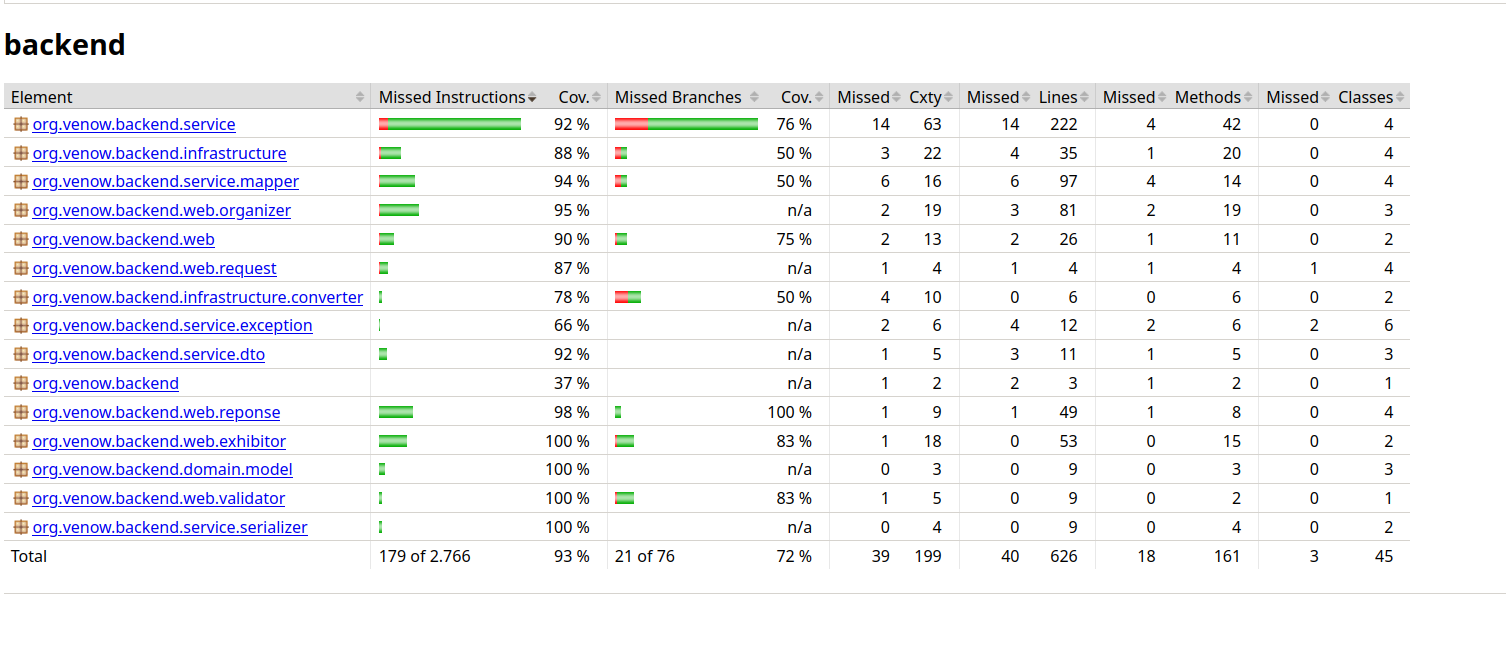
\includegraphics[width=1\textwidth]{fig/jacoco-honeycomb.png}
	\caption{Jacoco Honeycomb Testabdeckung}
	\label{fig:jacoco-honeycomb-full}
\end{figure}

\begin{figure}[h]
	\centering
	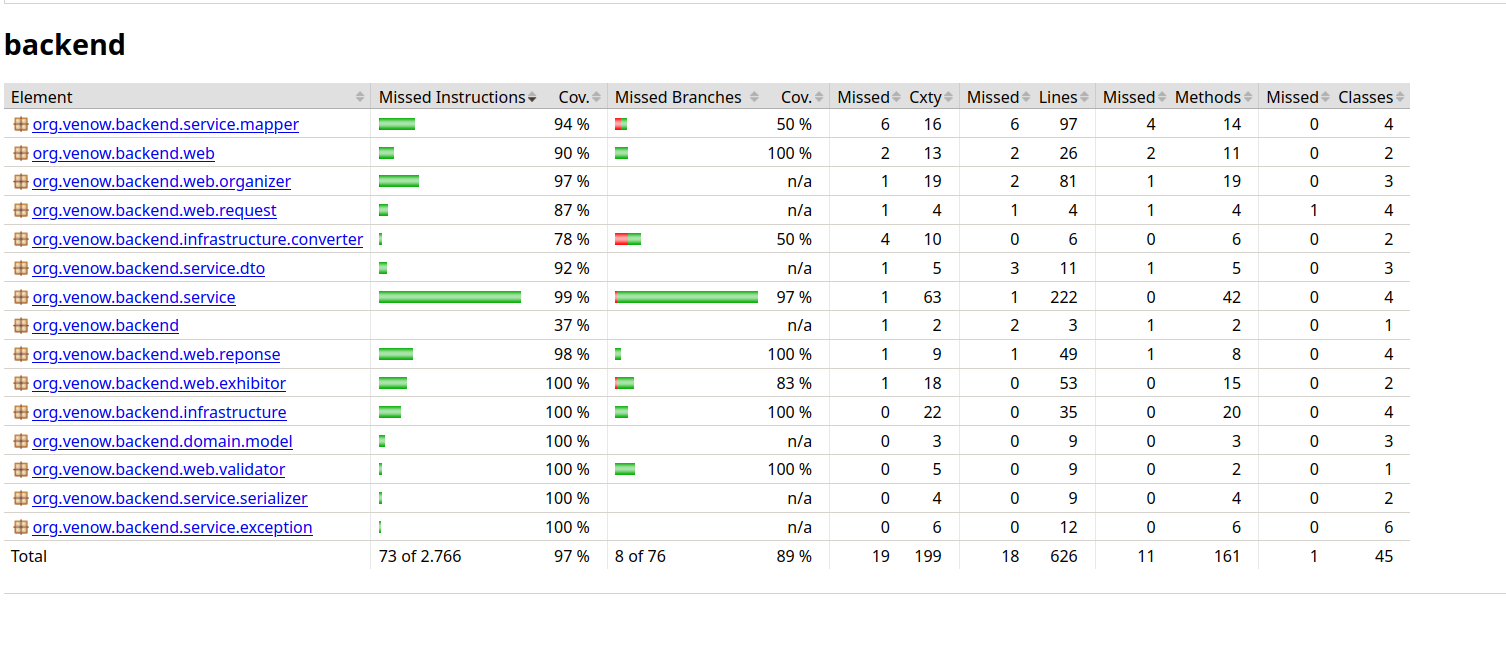
\includegraphics[width=1\textwidth]{fig/testpyrami-jacoco.png}
	\caption{Jacoco Testpyramid Testabdeckung}
	\label{fig:jacoco-testpyramid-full}
\end{figure}
\begin{figure}[h]
	\centering
	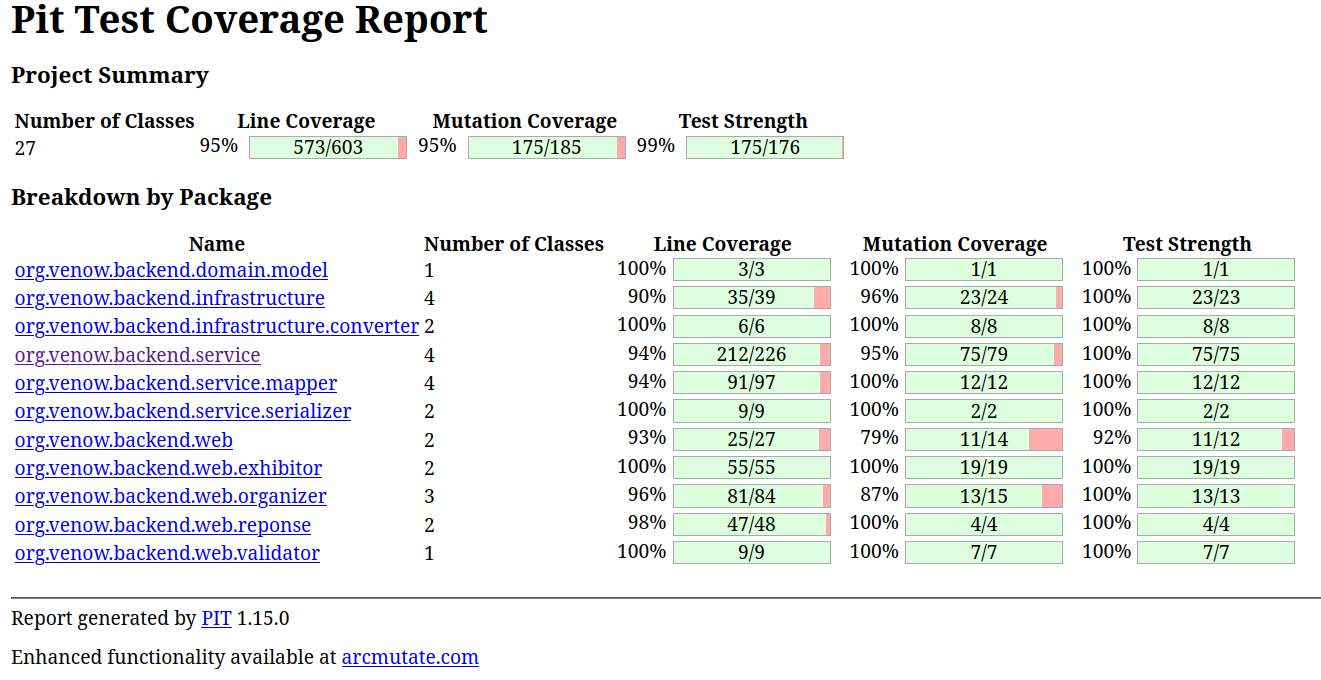
\includegraphics[width=1\textwidth]{fig/pitest-honeycomb.png}
	\caption{PIT - Mutation Honeycomb }
	\label{fig:pitest-honeycomb-full}
\end{figure}
\begin{figure}[h]
	\centering
	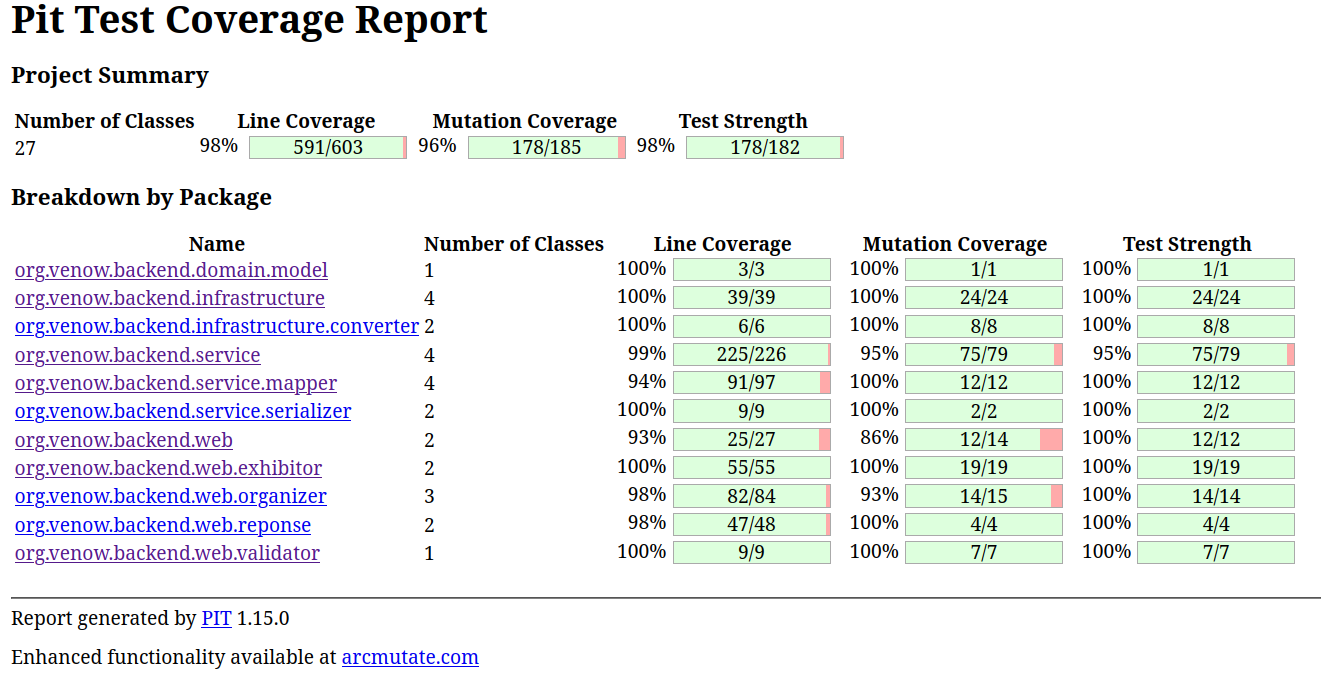
\includegraphics[width=1\textwidth]{fig/pitest-testpyramid.png}
	\caption{PIT - Mutation Testpyramid }
	\label{fig:pitest-testpyramid-full}
\end{figure}

%%%%%%%%%%%%%%%%%%%%%%%%%%%%%%%%%%%%%%%%%%%%%%%%%%%%%%%%%%%%%%%%%%%%%%%%%%%%%%%%
%% (Ende) Der Inhalt der Arbeit                                               %%
%%%%%%%%%%%%%%%%%%%%%%%%%%%%%%%%%%%%%%%%%%%%%%%%%%%%%%%%%%%%%%%%%%%%%%%%%%%%%%%%


\backmatter

\clearpage
\bibliography{references}
%% Depending on Language, use german alphadin or original alpha
\iflanguage{ngerman}{
  \bibliographystyle{alphadin}
}{
  \bibliographystyle{alpha}
}

\end{document}
